\section{Foundation\label{sec:foundation}}
In this chapter, the basic concepts fundamental to understanding the subject of the thesis will be explained. This allows a better understanding of the following chapters and the proposed solutions. Firstly, the foundations of systems engineering will be presented. Then the notions of \acrshort{cad}, \acrshort{cae}, and “Expert System” will be explained. This will be followed by an introduction to semantic technologies and an analysis of the use of semantic technologies in the field of systems engineering.\\



\subsection{System Engineering \label{sec:sysen}}
Systems engineering is a multidisciplinary approach to the design, implementation and management of complex systems throughout their life cycle (see Figure). It embraces a holistic perspective that takes into account the interactions and interdependencies between different components in order to achieve optimal performance and functionality. Systems engineering deals with work processes, optimisation methods and risk management tools in projects. Systems engineering ensures that all likely aspects of a project or system are considered and integrated as a whole. In the context of the automotive industry, where complex systems and simulations play a central role, the application of systems engineering principles becomes paramount.

\subsubsection{Core Concepts}
    The key principles of systems engineering are as follows:
    \begin{itemize}
      \item Requirements engineering: this phase consists of determining and documenting the needs and constraints that the system must satisfy. In the context of simulation configuration, understanding requirements is crucial to accurately model and simulate real-world automotive scenarios.
      
      \item System design: this phase involves transforming the requirements into a system plan. It involves assigning functions to components, taking into account factors such as efficiency, reliability, and maintainability. For simulation configuration, this step is essential to create a framework that aligns with the specific attributes of automotive simulations.
      
      \item Integration and testing: Systems engineering emphasizes the importance of rigorous testing and integration to ensure that all components work perfectly together. This is particularly relevant in the context of simulation configuration, where the accuracy and reliability of results depend on the effective integration of different simulation parameters.
      
      \item Lifecycle management: Systems engineering goes beyond the initial design and implementation phases. It involves continuous monitoring, maintenance and adaptation to changing requirements throughout the system's lifecycle. This perspective is crucial to the longevity and adaptability of simulation configurations in the dynamic automotive landscape.

    \end{itemize}

    
\subsubsection{V-Model}
The V-model illustrates systems development by highlighting the verification and validation stages. A graphical representation of this model is shown in Figure \ref{fig:v-model}. The system specification and detailed software design are presented on the left-hand side of the “V”, along with the steps leading to implementation. The steps mentioned on the left-hand side must be verified and validated on the right-hand side of the “V”. It also includes the integration of systems and software. Each step on the left is directly linked to a test step. Once the first stage has been successfully completed, the next stage begins.\\

\begin{figure}[H]
    \centering
    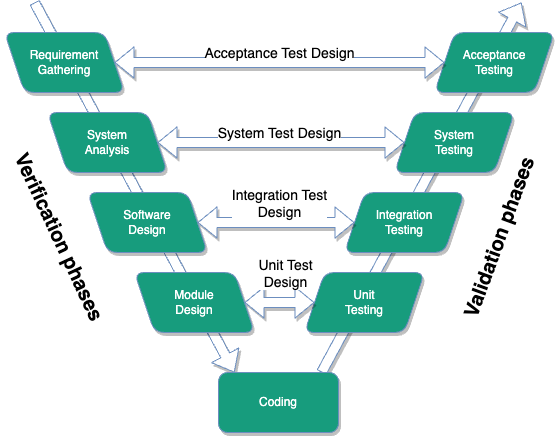
\includegraphics[scale=0.6]{images/V-Model.png}
    \caption{\label{fig:v-model} V-Model }
\end{figure}

With the evolution of technology, many software applications exist to cover these different stages more effectively. 

\subsection{\acrlong{cae} and Simulation}
\acrfull{cae}, also known as digital engineering or computer-aided engineering, brings together all the digital and software resources usually used by engineers to design, simulate, and validate new products and industrial processes using sophisticated algorithms. \acrshort{cae} tools enable the physical properties of a product to be tested and simulated so that it can be optimized based on the results of a numerical analysis.

    \subsubsection{Simulation-driven Design}
    Typically, \acrshort{cae} involves pre-processing, solving, and post-processing stages \cite{karlberg2013state}. During the pre-processing phase, engineers model the system, the physical properties of the design, and the operational environment in the form of applied constraints or loads. To correctly configure the resulting simulations, it is crucial that this modeling incorporates all parts of the environment to which the product will be exposed (including forces, temperatures, etc.).  The quality of the simulation is largely determined by the accuracy of the conditions to which the product will be exposed. Subsequently, the model is resolved through simulations prior to the presentation of the outcomes for evaluation during post-processing.\\

    Whereas physical prototyping takes days or even weeks, simulations take just a few hours at most. While physical prototyping is an inevitable process, the utilization of simulations can effectively mitigate the quantity of prototypes required prior to manufacturing \cite{sellgren1999simulation}.\\
    
    \textbf{Figure \ref{fig:v-model-sim}} shows the different types of simulations and tests throughout the “V” model presented above. Initial design and simulation of \acrfull{cad} geometry under appropriate conditions is the \acrshort{cae}'s standard workflow. Based on the results of the simulation, the design is improved. This process may need to be repeated until the product requirements are met and virtually confirmed. If there are differences in behavior between the digital prototype and expectations, the \acrshort{cad} model or input data can be adjusted \cite{sellgren1999simulation, jeon2016automatic}. This process speeds up product development because there is no need to create physical prototypes in the early stages of development.

    \begin{figure}[h]
        \centering
        \frame{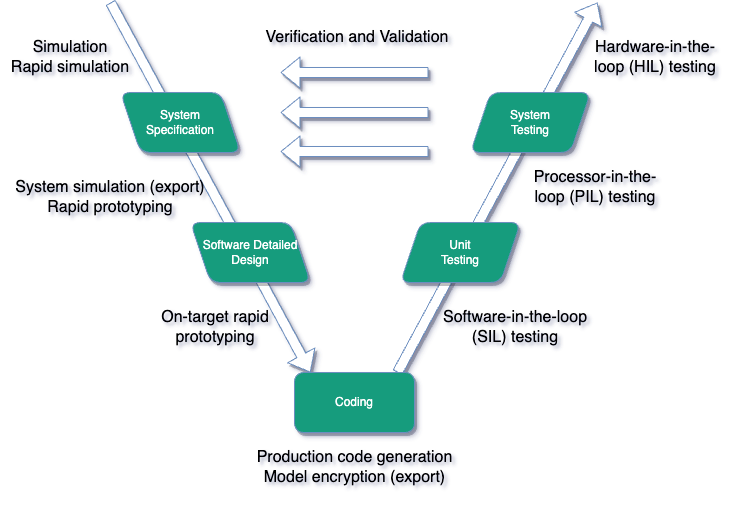
\includegraphics[scale=0.55]{images/Foundation-V-Model-Sim.drawio.png}}
        \caption[V-Model with Simulations]{\label{fig:v-model-sim} V-Model with Simulations \cite{validVerifSys} }
    \end{figure}


    \subsubsection{Advantages}
    One of the primary benefits of this methodology is in its expedited timeframe, as opposed to the protracted duration often required for constructing and evaluating tangible prototypes, which might span several days or even weeks. Of course, there will always be a need to build a physical prototype at some point, but \acrshort{cad} greatly reduces the number of prototypes required. The use of \acrshort{cad} and the resulting reduction in the need for physical prototypes means that product development costs and time can be reduced while guaranteeing better product quality.\\

    The benefits of \acrshort{cae} include
    \begin{itemize}
        \item Saving money: Compared to building several real prototypes, using computer simulations to evaluate designs is less expensive \cite{sellgren1999simulation}.
        \item Time savings: using \acrshort{cae} design tools means that designs can be created faster and more efficiently \cite{sellgren1999simulation}.
        \item Simple design editing: With \acrshort{cae}, editing a design is quick and easy. This allows you to correct errors and make changes to your design, enabling problems to be solved quickly and further savings to be made \cite{sellgren1999simulation}.
        \item Fewer errors: Compared with manual design, \acrshort{cad} can reduce the likelihood of errors \cite{sellgren1999simulation}.
        \item Less work: since \acrshort{cae} software automates a large part of the operation, designing various models requires less work \cite{sellgren1999simulation}.
        \item Less duplication of work: As the computer code is reusable, it is not necessary to perform the same activities several times. In addition, separate code segments can be duplicated and used during the design process \cite{sellgren1999simulation}.
        \item Easy to share: \acrshort{cae} design files can be easily saved and exchanged \cite{sellgren1999simulation, jeon2016automatic}.
        \item Greater accuracy: \acrshort{cad} software is more accurate than manual design, allowing you to work more precisely and achieve better results \cite{sellgren1999simulation}.
        \item Better decision-making: Performance impacts can guide design choices, and these impacts can be assessed early in the development phase when it is cheaper and simpler to make changes to the design \cite{sellgren1999simulation, validVerifSys}.
    \end{itemize}

    \subsubsection{Disadvantages}
    While \acrshort{cad} has many advantages, others argue that it is difficult to control the design of increasingly complicated components, as the correct results only appear later in the product design cycle \cite{karlberg2013state}. To overcome this difficulty, \acrshort{cae}'s software suppliers are constantly creating new tools and streamlining existing procedures. In addition, \acrshort{cad} can have the following disadvantages:

    \begin{itemize}
        \item Hardware Failure: A computer breakdown might result in job loss.
        \item Security: Work might be subject to hackers or viruses.
        \item Employee Competencies: Learning how to utilize the \acrshort{cae} program may require some training.
        \item System Expense: Purchasing new systems can be expensive.
        \item Updates: Recurrent system updates may be required.
    \end{itemize}

\subsection{Expert System\label{subsec:exp-sys}}
An expert system within the field of artificial intelligence refers to a computational program designed to replicate the cognitive processes involved in decision-making by a human expert \cite{liao2005expert, waterman1985guide}. It possesses knowledge in a given domain, extracted from the knowledge of experts in that domain.  Rather than using traditional procedural code, expert systems are designed to deal with complex questions posed by the user by reasoning from bodies of knowledge. The 1970s saw the development of the first expert systems, which came into widespread use in the 1980s \cite{buchanan1988fundamentals}. They were one of the first applications of \acrfull{ai} software to achieve real success \cite{buckley1986fuzzy, buchanan1988fundamentals, waterman1985guide}. \\

\textbf{Figure \ref{fig:es-archi}} shows the architecture of an expert system. An expert system consists of two subsystems: the knowledge base and the inference engine \cite{tripathi2011review}. Rules and information are represented in the knowledge base. The inference engine utilizes the rules to derive new facts from the existing facts. In addition, inference engines can be capable of debugging and explanation.\\

A non-expert user uses this software to gather information, while people who are experts in a given field enter data into the knowledge base. It is widely used in many fields, including coding, games, accounting, and medical diagnostics \cite{liao2005expert}. They can guide users and explain how they arrived at a specific recommendation or conclusion.\\

The process of creating an expert system is called \textbf{knowledge engineering}, and the people who carry it out are known as \textbf{knowledge engineers} \cite{waterman1985guide}. The main responsibility of the knowledge engineer is to ensure that the computer has all the knowledge it needs to solve a problem. To express the necessary information in the form of a symbolic model in the computer's memory, the knowledge engineer must choose one or more forms (the ontology will be chosen for this thesis).\\

\begin{figure}[h]
    \centering
    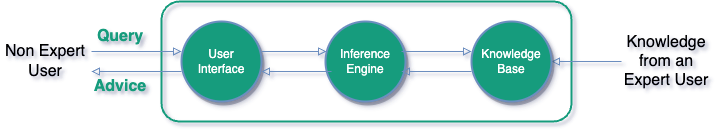
\includegraphics[scale=0.6]{images/Foundation-Architecture_Expert_System.drawio.png}
    \caption[Architecture of an Expert System]{\label{fig:es-archi} Architecture of an Expert System \cite{tripathi2011review} }
\end{figure}

\hfill \break

Components of an expert system : 
\begin{itemize}
    \item \textbf{Knowledge base}: Facts and rules are represented here. It is made up of intrinsic facts relevant to the domain, methods, rules for solving problems, and knowledge specific to the domain.
    \item \textbf{Inference engine}: this retrieves relevant information from the knowledge base, analyses it, and determines a solution that addresses the user's problem. To deduce new facts, the inference engine extracts rules from its knowledge base and applies them to known facts. In addition, debugging and explanation functions can be added to inference engines.
    \item \textbf{Learning and knowledge acquisition module}: This part aims to enable the expert system to collect and store knowledge from various sources on an ongoing basis.
    \item \textbf{User interface}: By utilizing this module, an individual lacking expertise can engage in communication with the expert system and collaboratively devise a resolution.
    \item \textbf{The explanation module} helps the expert system to provide the user with a detailed explanation of how it arrived at a certain result.
\end{itemize}


\subsection{Semantic Web\label{sec:semweb}}
The Semantic Web is an expansion of the World Wide Web that intends to enable robots to comprehend and interpret the meaning of content on the internet \cite{shadbolt2006semantic, berners2023semantic, kim2003semantic}. It entails encoding data in a way that improves interconnectivity, connecting similar information, and enabling computerized processing. The objective is to improve information retrieval efficiency while also enabling more intelligent online apps and services.\\

In 2001, Tim Berners-Lee coined the term “Semantic Web” to describe the use of semantic technologies in data connectivity \cite{berners2023semantic}. The World Wide Web Consortium (W3C), founded by Berners-Lee, disseminates and supports some technical guidelines for the Semantic Web.\\

Improving the way computers understand data makes it easier to share data and enables it to be processed automatically. As \textbf{Figure \ref{fig:sem-web-stack}} shows, the \acrfull{owl}, \acrfull{sparql}, and \acrfull{rdf} are the main standards on which semantic technology is developed. In contrast, in conventional information technology, meanings are hard-coded into application code and data at the design stage. \\

\begin{figure}[ht]
    \centering
    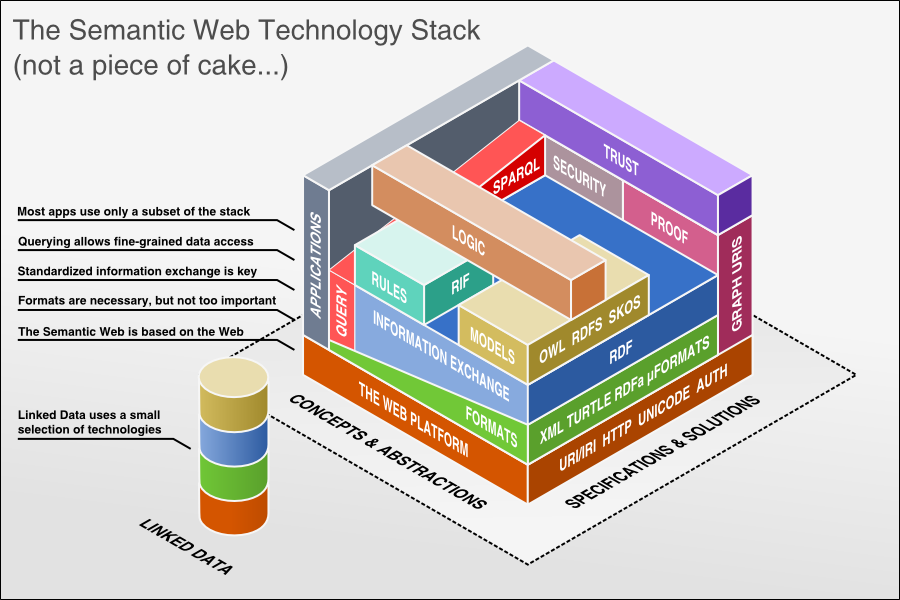
\includegraphics[scale=0.6]{images/foundation-sem-web-tech-stack.png}
    \caption[Semantic Web Technologies Stack]{\label{fig:sem-web-stack} Semantic Web Technologies Stack \cite{semWebStack} }
\end{figure}


    \subsubsection{\acrshort{uri} and \acrshort{iri}}
        \paragraph{\acrlong{uri}}
        A \acrfull{uri} is a short string of characters that identifies an abstract or physical resource on the Semantic Web \cite{de2016names}. The use of \acrshort{uri}s makes resources available through several naming systems and access mechanisms. A \acrshort{uri} can be used for location, identification, or both. There are two types of \acrshort{uri}: URLs and URNs. A \acrfull{url} is a specific type of \acrshort{uri} that specifies the location of a resource and provides instructions on how to access it. Conversely, an \acrfull{urn} is employed to designate an internet resource without explicitly indicating the method of retrieval.\\


        Semantic Web resource identifiers can be divided into a base \acrshort{uri} and a local name. In serialization, the base \acrshort{uri} is often shortened by a prefix defined at the beginning. \textbf{Figure  \ref{fig:uri-example}} shows an example of a \acrshort{uri} and its decomposition with a prefix. This figure shows that a \acrshort{uri} can be simplified by defining a prefix. We can see that a long \acrshort{uri} can be simplified and represented by \textbf{sim:LoadCase}.\\

        \begin{figure}[h]
            \centering
            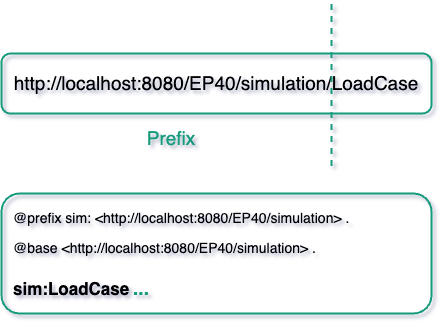
\includegraphics[scale=0.6]{images/Foundation-URI Decomposition.drawio.png}
            \caption{\label{fig:uri-example} Example of \acrshort{uri} and Decomposition with Prefix}
        \end{figure}

        
        \paragraph{\acrlong{iri}}
        \acrfull{iri} is an extension of the \acrshort{uri} that adapts to a global character set, whereas the \acrshort{uri} is limited to \acrshort{ascii} and has far fewer characters. \acrshort{iri}s enable the representation and communication of data-related knowledge in several languages. \acrshort{iri}s can be transformed into \acrshort{uri}s using percentage encoding, enabling backward compatibility.


    \subsubsection{\acrlong{rdf} \label{subsubsec:rdf}}
    \acrfull{rdf} is a resource description framework developed by W3C. It is used in particular on the World Wide Web for data exchange. The \acrshort{rdf} data model allows data resources to be uniquely recognized and linked to other data resources for reading, analysis, and action \textbf{\cite{decker2000framework}}. 

    \acrshort{rdf} introduces several fundamental Semantic Web terms:

    \begin{itemize}
        \item A \textbf{resource} is anything that can be characterized by an \acrshort{rdf} declaration. \acrshort{uri}s ensure that resources are always uniquely named. Any physical thing or notion can be represented by a \acrshort{uri}, allowing \acrshort{rdf} to be used to describe different types of domains.
        
        \item A \textbf{“thing”} is either an individual object, called an instance, or a definition of a type of thing, called a class. 
        
        \item A \textbf{schema} is an abstract description of a set of objects. It consists of a hierarchical taxonomy that describes how the elements of the domain are classified. In \acrshort{rdf}, schemas are also known as terminology boxes (Tboxes). 
        
        \item A \textbf{property} is an attribute, feature, characteristic, or connection that facilitates the description of a \acrshort{uri}. In the \acrshort{rdf} architecture, a property is also represented in the form of a \acrshort{uri}. It always has a precise meaning and determines the type of resource it can describe, known as the property domain, as well as the permitted values. It can also specify how it relates to other attributes. 
        
        \item \textbf{Axioms} are property declarations for schema classes, often known as Role Boxes (Rbox) in \acrshort{rdf}. They define the relationships between classes.
    \end{itemize}

    \acrshort{rdf} is a model based on \textbf{Triples}. Triples are built around \textbf{subject-predicate-object} relationships and are the most common type of axiom. The predicate is a property or a relation; the subject is a “thing”. When the object is a thing, the property is called an \textbf{object property}. If the object is a literal, such as a character, integer, or string, the property is called a \textbf{data property}. Once a triplet has been defined, it is referred to as a \textbf{statement} \cite{noy2001ontology}.\\

    Take, for example, this basic English sentence: “Germany is in Europe”. \textbf{Table \ref{tab:rdf-example}} shows how the sentence can be divided syntactically. If this statement were to be expressed visually, this could be done using the following directed graph, shown in \textbf{Figure \ref{fig:rdf-example}}.\\
    
    \begin{table}[h]
        \centering
	    \rowcolors{2}{teal!10}{white}
	    \begin{tabular}{ | m{4cm} | m{4cm} | m{4cm} | }
            \hline
            \rowcolor{teal!30} \textbf{Subject} & \textbf{Predicate} & \textbf{Object} \\
            
            \hline
            Germany  & is in & Europe\\
            
            \hline
        \end{tabular}
        \caption{\label{tab:rdf-example} RDF Syntactic Division}
        \end{table}
        
    \begin{figure}[h]
        \centering
        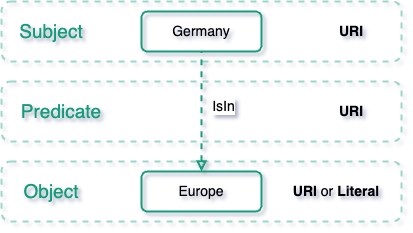
\includegraphics[scale=0.6]{images/Foundation-RDF Example.drawio.png}
        \caption{\label{fig:rdf-example}  RDF Graphical Representation}
    \end{figure}

    \acrshort{rdf} uses the same techniques to demonstrate the links between subjects and objects. However, as explained earlier, to represent resources and features accurately on the web, they need to be assigned a unique \acrshort{uri}. To demonstrate the representation of the above example sentence as a triple, the \acrshort{uri}s of the resources and attributes are assumed to be those shown in \textbf{Table \ref{tab:rdf-example-uri}}.
    
    \begin{table}[h]
        \centering
	    {\rowcolors{2}{teal!10}{white}
	    \begin{tabular}{ | m{2.5cm} | m{2.5cm} | c | }
            \hline
            \rowcolor{teal!30} \textbf{Entity} & \textbf{Role} & \textbf{URI} \\
            
            \hline
            Germany  & Subject & $<http://example/resource/Germany>$\\
            
            \hline
            is in  & Predicate & $<http://example/resource/isIn>$\\
            
            \hline
            Europe  & Object & $<http://example/resource/Europe>$\\
            
            \hline
        \end{tabular}}
        \caption{\label{tab:rdf-example-uri} Example of URI Scheme}
    \end{table}

    \subsubsection{Linked Data Principles}
    Linked data is a way of representing and distributing structured data on the web. Data generated and structured according to Linked Data principles is machine-readable and connected to other data on the web. It uses conventional web technologies such as \acrshort{http}, \acrshort{rdf}, and \acrshort{uri}, but not only does it provide human-readable data via web pages, it also makes it machine-readable \cite{bizer2008linked}. Linked data allows concepts, elements, events, people, places, etc. to be organized and linked together. Many platforms on the web make available a large amount of linked data and the relationships between them. These include WikiData, DBpedia, and \acrfull{lov}.\\

    Tim Berners-Lee, the initiator and defender of the Semantic Web and linked data, established the four design principles of linked data back in 2006 \cite{bizer2008linked, bizer2011linked}.
    \begin{enumerate}
        \item Use \acrshort{uri}s to name objects.
        \item Use \acrshort{http} \acrshort{uri}s to provide useful information. 
        \item Use open standards such as \acrshort{rdf} and \acrshort{sparql} to provide meaningful information about what a name indicates when searched. 
        \item Include connections to other \acrshort{uri}s to allow them to find new information. 
    \end{enumerate}

    The more data is represented as linked data on the web, the greater the possibility of linking it to other linked data sources. For example, if a resource represented by an \acrshort{uri} in one data source is discovered in an existing linked data source (e.g., WikiData or DBpedia), it can be connected to a property such as \textbf{owl:sameAs} to extract further metadata and investigate links to other data resources \cite{bizer2008linked}.\\

    \subsubsection{Ontology \label{subsubsec:ontology}}
    In the field of philosophy, ontology is a discipline that studies existence, and how knowledge, language, and perception are related to the nature of reality \cite{smith2012ontology}. It is concerned with the question of what entities exist and how they can be classified, ordered hierarchically, and discriminated against. \\
    Since the mid-1970s, \acrshort{ai} researchers have realized that knowledge engineering is essential for developing large and powerful \acrshort{ai} systems \cite{fensel2001ontologies}. \acrshort{ai} researchers suggested that they could develop new ontologies as computational models to enable certain types of automated reasoning, but their efforts were only moderately successful. In the 1980s, the \acrshort{ai} community began using the term ontology to describe both a theory of a modeled world and a component of knowledge-based systems \cite{guarino1995formal}.\\
    An ontology captures the structure of a domain, i.e., the model and its constraints. In other words, an ontology is a structure for systematically storing and formalizing domain knowledge. Ontology schemas are created using two modeling languages, \acrfull{rdfs} and \acrfull{owl} \cite{fensel2001ontologies}.\\

    Tim Berners-Lee \cite{kuck2004tim} defines an ontology as having the following properties: 
    \begin{enumerate}
        \item It must have a concise syntax.
        \item It must have well-defined semantics, making it possible to state correctly what is represented.
        \item It must have sufficient expressive capacity to convey human knowledge.
        \item It must have an effective, robust, and simple reasoning process. 5. it must be capable of generating huge knowledge bases.
    \end{enumerate}


\subsection{Role of Semantic Technology in Systems Engineering}
To improve the efficiency of systems engineering processes, the integration of semantic technology appears to be a promising avenue \cite{hagedorn2020knowledge}. The application of semantic technology to simulation configuration in the automotive industry provides a more nuanced understanding of the relationships between simulation parameters, facilitating intelligent decision-making and configuration suggestions. Using \acrshort{rdf} standards, the metadata of many artifacts in a simulation can be merged into a single database. The database will include objects and information useful throughout the configuration process, uniformly represented as \acrshort{rdf} graphs. This integration allows \acrshort{sparql} to query the database, enabling complex queries to be managed.\\

This study aims to bridge the gap between traditional systems engineering methodologies and cutting-edge semantic technologies, providing a new perspective on the configuration processes that are essential for advancing simulation capabilities in the automotive sector. In the next chapter, an analysis of the “State of the Art” and “of Practice” will be made to have a more precise idea of the work already done on this subject.











